\section{Utility and System Functions and Macros}

\ifCPy
\cvfunc{Error Handling}\label{Error handling}

\ifPy
Errors in argument type cause a \texttt{TypeError} exception.
OpenCV errors cause a cv.error exception.
\fi

\ifC
Error handling in OpenCV is similar to IPL (Image Processing
Library). In the case of an error, functions do not return the error
code. Instead, they raise an error using \texttt{CV\_ERROR}
macro that calls \cvCPyCross{Error} that, in its turn, sets the error
status with \cvCPyCross{SetErrStatus} and calls a standard or user-defined
error handler (that can display a message box, write to log, etc., see
\cvCPyCross{RedirectError}).  There is a global variable, one per each program
thread, that contains current error status (an integer value). The status
can be retrieved with the \cvCPyCross{GetErrStatus} function.

There are three modes of error handling (see \cvCPyCross{SetErrMode} and
\cvCPyCross{GetErrMode}):

\begin{description}
\cvarg{Leaf}{The program is terminated after the error handler is
called. This is the default value. It is useful for debugging, as the
error is signalled immediately after it occurs. However, for production
systems, other two methods may be preferable as they provide more
control.}
\cvarg{Parent}{The program is not terminated, but the error handler
is called. The stack is unwound (it is done w/o using a C++ exception
mechanism). The user may check error code after calling the \texttt{CxCore} function with
\cvCPyCross{GetErrStatus} and react.}
\cvarg{Silent}{Similar to \texttt{Parent} mode, but no error handler
is called}
\end{description}

Actually, the semantics of the \texttt{Leaf} and \texttt{Parent} modes are implemented by error handlers and the above description is true for them. \cvCPyCross{GuiBoxReport} behaves slightly differently, and some custom error handlers may implement quite different semantics.  

Macros for raising an error, checking for errors, etc.
\begin{lstlisting}

/* special macros for enclosing processing statements within a function and separating
   them from prologue (resource initialization) and epilogue (guaranteed resource release) */
#define __BEGIN__       {
#define __END__         goto exit; exit: ; }
/* proceeds to "resource release" stage */
#define EXIT            goto exit

/* Declares locally the function name for CV_ERROR() use */
#define CV_FUNCNAME( Name )  \
    static char cvFuncName[] = Name

/* Raises an error within the current context */
#define CV_ERROR( Code, Msg )                                       \
{                                                                   \
     cvError( (Code), cvFuncName, Msg, __FILE__, __LINE__ );        \
     EXIT;                                                          \
}

/* Checks status after calling CXCORE function */
#define CV_CHECK()                                                  \
{                                                                   \
    if( cvGetErrStatus() < 0 )                                   \
        CV_ERROR( CV_StsBackTrace, "Inner function failed." );      \
}

/* Provies shorthand for CXCORE function call and CV_CHECK() */
#define CV_CALL( Statement )                                        \
{                                                                   \
    Statement;                                                      \
    CV_CHECK();                                                     \
}

/* Checks some condition in both debug and release configurations */
#define CV_ASSERT( Condition )                                          \
{                                                                       \
    if( !(Condition) )                                                  \
        CV_ERROR( CV_StsInternal, "Assertion: " #Condition " failed" ); \
}

/* these macros are similar to their CV_... counterparts, but they
   do not need exit label nor cvFuncName to be defined */
#define OPENCV_ERROR(status,func_name,err_msg) ...
#define OPENCV_ERRCHK(func_name,err_msg) ...
#define OPENCV_ASSERT(condition,func_name,err_msg) ...
#define OPENCV_CALL(statement) ...

\end{lstlisting}

Instead of a discussion, below is a documented example of a typical CXCORE function and an example of the function use.

\cvfunc{Example: Use of Error Handling Macros}
\begin{lstlisting}

#include "cxcore.h"
#include <stdio.h>

void cvResizeDCT( CvMat* input_array, CvMat* output_array )
{
    CvMat* temp_array = 0; // declare pointer that should be released anyway.

    CV_FUNCNAME( "cvResizeDCT" ); // declare cvFuncName

    __BEGIN__; // start processing. There may be some declarations just after 
              // this macro, but they could not be accessed from the epilogue.

    if( !CV_IS_MAT(input_array) || !CV_IS_MAT(output_array) )
        // use CV_ERROR() to raise an error
        CV_ERROR( CV_StsBadArg, 
	"input_array or output_array are not valid matrices" );

    // some restrictions that are going to be removed later, may be checked 
    // with CV_ASSERT()
    CV_ASSERT( input_array->rows == 1 && output_array->rows == 1 );

    // use CV_CALL for safe function call
    CV_CALL( temp_array = cvCreateMat( input_array->rows,
                                       MAX(input_array->cols,
				       output_array->cols),
                                       input_array->type ));

    if( output_array->cols > input_array->cols )
        CV_CALL( cvZero( temp_array ));

    temp_array->cols = input_array->cols;
    CV_CALL( cvDCT( input_array, temp_array, CV_DXT_FORWARD ));
    temp_array->cols = output_array->cols;
    CV_CALL( cvDCT( temp_array, output_array, CV_DXT_INVERSE ));
    CV_CALL( cvScale( output_array,
                      output_array,
                      1./sqrt((double)input_array->cols*output_array->cols), 0 ));

    __END__; // finish processing. Epilogue follows after the macro.

    // release temp_array. If temp_array has not been allocated
    // before an error occured, cvReleaseMat
    // takes care of it and does nothing in this case.
    cvReleaseMat( &temp_array );
}

int main( int argc, char** argv )
{
    CvMat* src = cvCreateMat( 1, 512, CV_32F );
#if 1 /* no errors */
    CvMat* dst = cvCreateMat( 1, 256, CV_32F );
#else
    CvMat* dst = 0; /* test error processing mechanism */
#endif
    cvSet( src, cvRealScalar(1.), 0 );
#if 0 /* change 0 to 1 to suppress error handler invocation */
    cvSetErrMode( CV_ErrModeSilent );
#endif
    cvResizeDCT( src, dst ); // if some error occurs, the message
                             // box will popup, or a message will be
                             // written to log, or some user-defined
                             // processing will be done
    if( cvGetErrStatus() < 0 )
        printf("Some error occured" );
    else
        printf("Everything is OK" );
    return 0;
}
\end{lstlisting}

\cvCPyFunc{GetErrStatus}
Returns the current error status.

\cvcodeC{int cvGetErrStatus( void );}

The function returns the current error status -
the value set with the last \cvCPyCross{SetErrStatus} call. Note that in
\texttt{Leaf} mode, the program terminates immediately after an
error occurs, so to always gain control after the function call,
one should call \cvCPyCross{SetErrMode} and set the \texttt{Parent}
or \texttt{Silent} error mode.

\cvCPyFunc{SetErrStatus}
Sets the error status.

\cvcodeC{void cvSetErrStatus( int status );}

\begin{description}
\cvarg{status}{The error status}
\end{description}

The function sets the error status to the specified value. Mostly, the function is used to reset the error status (set to it \texttt{CV\_StsOk}) to recover after an error. In other cases it is more natural to call \cvCPyCross{Error} or \texttt{CV\_ERROR}.

\cvCPyFunc{GetErrMode}
Returns the current error mode.

\cvcodeC{int cvGetErrMode(void);}

The function returns the current error mode - the value set with the last \cvCPyCross{SetErrMode} call.

\cvCPyFunc{SetErrMode}
Sets the error mode.

\begin{lstlisting}
#define CV_ErrModeLeaf    0
#define CV_ErrModeParent  1
#define CV_ErrModeSilent  2
\end{lstlisting}

\cvcodeC{int cvSetErrMode( int mode );}

\begin{description}
\cvarg{mode}{The error mode}
\end{description}

The function sets the specified error mode. For descriptions of different error modes, see the beginning of the error section.

\cvCPyFunc{Error}
Raises an error.

\cvcodeC{int cvError( \par int status,\par const char* func\_name,\par const char* err\_msg,\par const char* filename,\par int line );}

\begin{description}
\cvarg{status}{The error status}
\cvarg{func\_name}{Name of the function where the error occured}
\cvarg{err\_msg}{Additional information/diagnostics about the error}
\cvarg{filename}{Name of the file where the error occured}
\cvarg{line}{Line number, where the error occured}
\end{description}

The function sets the error status to the specified value (via \cvCPyCross{SetErrStatus}) and, if the error mode is not \texttt{Silent}, calls the error handler.

\cvCPyFunc{ErrorStr}
Returns textual description of an error status code.

\cvcodeC{const char* cvErrorStr( int status );}

\begin{description}
\cvarg{status}{The error status}
\end{description}

The function returns the textual description for
the specified error status code. In the case of unknown status, the function
returns a NULL pointer.

\cvCPyFunc{RedirectError}
Sets a new error handler.

\begin{lstlisting}
typedef int (CV_CDECL *CvErrorCallback)( int status, const char* func_name,
                    const char* err_msg, const char* file_name, int line );
\end{lstlisting}

\cvcodeC{CvErrorCallback cvRedirectError( \par CvErrorCallback error\_handler,\par void* userdata=NULL,\par void** prevUserdata=NULL );}

\begin{description}
\cvarg{error\_handler}{The new error\_handler}
\cvarg{userdata}{Arbitrary pointer that is transparently passed to the error handler}
\cvarg{prevUserdata}{Pointer to the previously assigned user data pointer}
\end{description}

The function sets a new error handler that
can be one of the standard handlers or a custom handler
that has a specific interface. The handler takes the same parameters
as the \cvCPyCross{Error} function. If the handler returns a non-zero value, the
program is terminated; otherwise, it continues. The error handler may
check the current error mode with \cvCPyCross{GetErrMode} to make a decision.


\cvfunc{cvNulDevReport cvStdErrReport cvGuiBoxReport}
\label{cvNulDevReport}
\label{cvStdErrReport}
\label{cvGuiBoxReport}

Provide standard error handling.

\begin{lstlisting}
int cvNulDevReport( int status, const char* func_name,
                    const char* err_msg, const char* file_name,
                    int line, void* userdata );

int cvStdErrReport( int status, const char* func_name,
                    const char* err_msg, const char* file_name,
                    int line, void* userdata );

int cvGuiBoxReport( int status, const char* func_name,
                    const char* err_msg, const char* file_name,
                    int line, void* userdata );
\end{lstlisting}

\begin{description}
\cvarg{status}{The error status}
\cvarg{func\_name}{Name of the function where the error occured}
\cvarg{err\_msg}{Additional information/diagnostics about the error}
\cvarg{filename}{Name of the file where the error occured}
\cvarg{line}{Line number, where the error occured}
\cvarg{userdata}{Pointer to the user data. Ignored by the standard handlers}
\end{description}

The functions \texttt{cvNullDevReport}, \texttt{cvStdErrReport},
and \texttt{cvGuiBoxReport} provide standard error
handling. \texttt{cvGuiBoxReport} is the default error
handler on Win32 systems, \texttt{cvStdErrReport} is the default on other
systems. \texttt{cvGuiBoxReport} pops up a message box with the error
description and suggest a few options. Below is an example message box
that may be recieved with the sample code above, if one introduces an
error as described in the sample.

\textbf{Error Message Box}
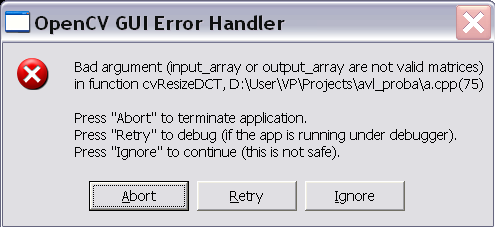
\includegraphics[width=0.5\textwidth]{pics/errmsg.png}

If the error handler is set to \texttt{cvStdErrReport}, the above message will be printed to standard error output and the program will be terminated or continued, depending on the current error mode.

\textbf{Error Message printed to Standard Error Output (in \texttt{Leaf} mode)}

\begin{verbatim}
OpenCV ERROR: Bad argument (input_array or output_array are not valid matrices)
        in function cvResizeDCT, D:\User\VP\Projects\avl\_proba\a.cpp(75)
Terminating the application...
\end{verbatim}

\cvCPyFunc{Alloc}
Allocates a memory buffer.

\cvcodeC{void* cvAlloc( size\_t size );}

\begin{description}
\cvarg{size}{Buffer size in bytes}
\end{description}

The function allocates \texttt{size} bytes and returns
a pointer to the allocated buffer. In the case of an error the function reports an
error and returns a NULL pointer. By default, \texttt{cvAlloc} calls
\texttt{icvAlloc} which
itself calls \texttt{malloc}. However it is possible to assign user-defined memory
allocation/deallocation functions using the \cvCPyCross{SetMemoryManager} function.

\cvCPyFunc{Free}
Deallocates a memory buffer.

\cvcodeC{void cvFree( void** ptr );}

\begin{description}
\cvarg{ptr}{Double pointer to released buffer}
\end{description}

The function deallocates a memory buffer allocated by
\cvCPyCross{Alloc}. It clears the pointer to buffer upon exit, which is why
the double pointer is used. If the \texttt{*buffer} is already NULL, the function
does nothing.

\cvCPyFunc{GetTickCount}
Returns the number of ticks.

\cvcodeC{int64 cvGetTickCount( void );}

The function returns number of the ticks starting from some platform-dependent event (number of CPU ticks from the startup, number of milliseconds from 1970th year, etc.). The function is useful for accurate measurement of a function/user-code execution time. To convert the number of ticks to time units, use \cvCPyCross{GetTickFrequency}.

\cvCPyFunc{GetTickFrequency}
Returns the number of ticks per microsecond.

\cvcodeC{double cvGetTickFrequency( void );}

The function returns the number of ticks per microsecond. Thus, the quotient of \cvCPyCross{GetTickCount} and \cvCPyCross{GetTickFrequency} will give the number of microseconds starting from the platform-dependent event.

\cvCPyFunc{RegisterModule}
Registers another module.

\begin{lstlisting}
typedef struct CvPluginFuncInfo
{
    void** func_addr;
    void* default_func_addr;
    const char* func_names;
    int search_modules;
    int loaded_from;
}
CvPluginFuncInfo;

typedef struct CvModuleInfo
{
    struct CvModuleInfo* next;
    const char* name;
    const char* version;
    CvPluginFuncInfo* func_tab;
}
CvModuleInfo;
\end{lstlisting}

\cvcodeC{int cvRegisterModule( const CvModuleInfo* moduleInfo );}

\begin{description}
\cvarg{moduleInfo}{Information about the module}
\end{description}

The function adds a module to the list of
registered modules. After the module is registered, information about
it can be retrieved using the \cvCPyCross{GetModuleInfo} function. Also, the
registered module makes full use of optimized plugins (IPP, MKL, ...),
supported by CXCORE. CXCORE itself, CV (computer vision), CVAUX (auxilary
computer vision), and HIGHGUI (visualization and image/video acquisition) are
examples of modules. Registration is usually done when the shared library
is loaded. See \texttt{cxcore/src/cxswitcher.cpp} and
\texttt{cv/src/cvswitcher.cpp} for details about how registration is done
and look at \texttt{cxcore/src/cxswitcher.cpp}, \texttt{cxcore/src/\_cxipp.h}
on how IPP and MKL are connected to the modules.

\cvCPyFunc{GetModuleInfo}
Retrieves information about registered module(s) and plugins.

\cvcodeC{
void  cvGetModuleInfo( \par const char* moduleName,\par const char** version,\par const char** loadedAddonPlugins);
}

\begin{description}
\cvarg{moduleName}{Name of the module of interest, or NULL, which means all the modules}
\cvarg{version}{The output parameter. Information about the module(s), including version}
\cvarg{loadedAddonPlugins}{The list of names and versions of the optimized plugins that CXCORE was able to find and load}
\end{description}

The function returns information about one or
all of the registered modules. The returned information is stored inside
the libraries, so the user should not deallocate or modify the returned
text strings.

\cvCPyFunc{UseOptimized}
Switches between optimized/non-optimized modes.

\cvcodeC{int cvUseOptimized( int onoff );}

\begin{description}
\cvarg{onoff}{Use optimized ($\ne 0$) or not ($=0$)}
\end{description}

The function switches between the mode, where
only pure C implementations from cxcore, OpenCV, etc. are used, and
the mode, where IPP and MKL functions are used if available. When
\texttt{cvUseOptimized(0)} is called, all the optimized libraries are
unloaded. The function may be useful for debugging, IPP and MKL upgrading on
the fly, online speed comparisons, etc. It returns the number of optimized
functions loaded. Note that by default, the optimized plugins are loaded,
so it is not necessary to call \texttt{cvUseOptimized(1)} in the beginning of
the program (actually, it will only increase the startup time).

\cvCPyFunc{SetMemoryManager}
Accesses custom/default memory managing functions.

\begin{lstlisting}
typedef void* (CV_CDECL *CvAllocFunc)(size_t size, void* userdata);
typedef int (CV_CDECL *CvFreeFunc)(void* pptr, void* userdata);
\end{lstlisting}

\cvcodeC{
void cvSetMemoryManager( \par CvAllocFunc allocFunc=NULL,\par CvFreeFunc freeFunc=NULL,\par void* userdata=NULL );
}

\begin{description}
\cvarg{allocFunc}{Allocation function; the interface is similar to \texttt{malloc}, except that \texttt{userdata} may be used to determine the context}
\cvarg{freeFunc}{Deallocation function; the interface is similar to \texttt{free}}
\cvarg{userdata}{User data that is transparently passed to the custom functions}
\end{description}

The function sets user-defined memory
managment functions (substitutes for \texttt{malloc} and \texttt{free}) that will be called
by \texttt{cvAlloc, cvFree} and higher-level functions (e.g., \texttt{cvCreateImage}). Note
that the function should be called when there is data allocated using
\texttt{cvAlloc}. Also, to avoid infinite recursive calls, it is not
allowed to call \texttt{cvAlloc} and \cvCPyCross{Free} from the custom
allocation/deallocation functions.

If the \texttt{alloc\_func} and \texttt{free\_func} pointers are
\texttt{NULL}, the default memory managing functions are restored.

\cvCPyFunc{SetIPLAllocators}
Switches to IPL functions for image allocation/deallocation.

\begin{lstlisting}
typedef IplImage* (CV_STDCALL* Cv_iplCreateImageHeader)
                            (int,int,int,char*,char*,int,int,int,int,int,
                            IplROI*,IplImage*,void*,IplTileInfo*);
typedef void (CV_STDCALL* Cv_iplAllocateImageData)(IplImage*,int,int);
typedef void (CV_STDCALL* Cv_iplDeallocate)(IplImage*,int);
typedef IplROI* (CV_STDCALL* Cv_iplCreateROI)(int,int,int,int,int);
typedef IplImage* (CV_STDCALL* Cv_iplCloneImage)(const IplImage*);

#define CV_TURN_ON_IPL_COMPATIBILITY()                                  \
    cvSetIPLAllocators( iplCreateImageHeader, iplAllocateImage,         \
                        iplDeallocate, iplCreateROI, iplCloneImage )
\end{lstlisting}

\cvcodeC{
void cvSetIPLAllocators( \par
                         Cv\_iplCreateImageHeader create\_header, \par
                         Cv\_iplAllocateImageData allocate\_data, \par
                         Cv\_iplDeallocate deallocate, \par
                         Cv\_iplCreateROI create\_roi, \par
                         Cv\_iplCloneImage clone\_image );
}

\begin{description}
\cvarg{create\_header}{Pointer to iplCreateImageHeader}
\cvarg{allocate\_data}{Pointer to iplAllocateImage}
\cvarg{deallocate}{Pointer to iplDeallocate}
\cvarg{create\_roi}{Pointer to iplCreateROI}
\cvarg{clone\_image}{Pointer to iplCloneImage}
\end{description}


The function causes CXCORE to use IPL functions
for image allocation/deallocation operations. For convenience, there
is the wrapping macro \texttt{CV\_TURN\_ON\_IPL\_COMPATIBILITY}. The
function is useful for applications where IPL and CXCORE/OpenCV are used
together and still there are calls to \texttt{iplCreateImageHeader},
etc. The function is not necessary if IPL is called only for data
processing and all the allocation/deallocation is done by CXCORE, or
if all the allocation/deallocation is done by IPL and some of OpenCV
functions are used to process the data.

\fi

\fi

\ifCpp

\cvCppFunc{alignPtr}
Aligns pointer to the specified number of bytes

\begin{lstlisting}
template<typename _Tp> _Tp* alignPtr(_Tp* ptr, int n=sizeof(_Tp));
\end{lstlisting}
\begin{description}
\cvarg{ptr}{The aligned pointer}
\cvarg{n}{The alignment size; must be a power of two}
\end{description}

The function returns the aligned pointer of the same type as the input pointer:
\[\texttt{(\_Tp*)(((size\_t)ptr + n-1) \& -n)}\]


\cvCppFunc{alignSize}
Aligns a buffer size to the specified number of bytes

\begin{lstlisting}
size_t alignSize(size_t sz, int n);
\end{lstlisting}
\begin{description}
\cvarg{sz}{The buffer size to align}
\cvarg{n}{The alignment size; must be a power of two}
\end{description}

The function returns the minimum number that is greater or equal to \texttt{sz} and is divisble by \texttt{n}:
\[\texttt{(sz + n-1) \& -n}\]


\cvCppFunc{allocate}
Allocates an array of elements

\begin{lstlisting}
template<typename _Tp> _Tp* allocate(size_t n);
\end{lstlisting}
\begin{description}
\cvarg{n}{The number of elements to allocate}
\end{description}

The generic function \texttt{allocate} allocates buffer for the specified number of elements. For each element the default constructor is called.


\cvCppFunc{deallocate}
Allocates an array of elements

\begin{lstlisting}
template<typename _Tp> void deallocate(_Tp* ptr, size_t n);
\end{lstlisting}
\begin{description}
\cvarg{ptr}{Pointer to the deallocated buffer}
\cvarg{n}{The number of elements in the buffer}
\end{description}

The generic function \texttt{deallocate} deallocates the buffer allocated with \cvCppCross{allocate}. The number of elements must match the number passed to \cvCppCross{allocate}.

\cvfunc{CV\_Assert}\label{CV Assert}
Checks a condition at runtime.

\begin{lstlisting}
#define CV_Assert( expr ) ...
#define CV_DbgAssert(expr) ...
\end{lstlisting}

\begin{description}
\cvarg{expr}{The checked expression}
\end{description}

The macros \texttt{CV\_Assert} and \texttt{CV\_DbgAssert} evaluate the specified expression and if it is 0, the macros raise an error (see \cvCppCross{error}). The macro \texttt{CV\_Assert} checks the condition in both Debug and Release configurations, while \texttt{CV\_DbgAssert} is only retained in the Debug configuration.

\cvCppFunc{error}
Signals an error and raises the exception

\begin{lstlisting}
void error( const Exception& exc );

#define CV_Error( code, msg )
#define CV_Error_( code, args )
\end{lstlisting}
\begin{description}
\cvarg{exc}{The exception to throw}
\cvarg{code}{The error code, normally, a negative value. The list of pre-defined error codes can be found in \texttt{cxerror.h}}
\cvarg{msg}{Text of the error message}
\cvarg{args}{printf-like formatted error message in parantheses}
\end{description}

The function and the helper macros \texttt{CV\_Error} and \texttt{CV\_Error\_} call the error handler. Currently, the error handler prints the error code (\texttt{exc.code}), the context (\texttt{exc.file}, \texttt{exc.line} and the error message \texttt{exc.err} to the standard error stream \texttt{stderr}. In Debug configuration it then provokes memory access violation, so that the execution stack and all the parameters can be analyzed in debugger. In Release configuration the exception \texttt{exc} is thrown.

The macro \texttt{CV\_Error\_} can be used to construct the error message on-fly to include some dynamic information, for example:

\begin{lstlisting}
// note the extra parentheses around the formatted text message
CV_Error_(CV_StsOutOfRange,
    ("the matrix element (%d,%d)=%g is out of range",
    i, j, mtx.at<float>(i,j)))
\end{lstlisting}


\cvCppFunc{Exception}
The exception class passed to error

\begin{lstlisting}
class  Exception
{
public:
    // various constructors and the copy operation
    Exception() { code = 0; line = 0; }
    Exception(int _code, const string& _err,
              const string& _func, const string& _file, int _line);
    Exception(const Exception& exc);
    Exception& operator = (const Exception& exc);

    // the error code
    int code;
    // the error text message
    string err;
    // function name where the error happened
    string func;
    // the source file name where the error happened
    string file;
    // the source file line where the error happened
    int line;
};
\end{lstlisting}

The class \texttt{Exception} encapsulates all or almost all the necessary information about the error happened in the program. The exception is usually constructed and thrown implicitly, via \texttt{CV\_Error} and \texttt{CV\_Error\_} macros, see \cvCppCross{error}.


\cvCppFunc{fastMalloc}
Allocates aligned memory buffer

\begin{lstlisting}
void* fastMalloc(size_t size);
\end{lstlisting}
\begin{description}
\cvarg{size}{The allocated buffer size}
\end{description}
 
The function allocates buffer of the specified size and returns it. When the buffer size is 16 bytes or more, the returned buffer is aligned on 16 bytes.

\cvCppFunc{fastFree}
Deallocates memory buffer

\begin{lstlisting}
void fastFree(void* ptr);
\end{lstlisting}
\begin{description}
\cvarg{ptr}{Pointer to the allocated buffer}
\end{description}

The function deallocates the buffer, allocated with \cvCppCross{fastMalloc}.
If NULL pointer is passed, the function does nothing.

\cvCppFunc{format}
Returns a text string formatted using printf-like expression

\begin{lstlisting}
string format( const char* fmt, ... );
\end{lstlisting}
\begin{description}
\cvarg{fmt}{The printf-compatible formatting specifiers}
\end{description}

The function acts like \texttt{sprintf}, but forms and returns STL string. It can be used for form the error message in \cvCppCross{Exception} constructor.

\cvCppFunc{getNumThreads}
Returns the number of threads used by OpenCV

\begin{lstlisting}
int getNumThreads();
\end{lstlisting}

The function returns the number of threads that is used by OpenCV.

See also: \cvCppCross{setNumThreads}, \cvCppCross{getThreadNum}.


\cvCppFunc{getThreadNum}
Returns index of the currently executed thread

\begin{lstlisting}
int getThreadNum();
\end{lstlisting}

The function returns 0-based index of the currently executed thread. The function is only valid inside a parallel OpenMP region. When OpenCV is built without OpenMP support, the function always returns 0.

See also: \cvCppCross{setNumThreads}, \cvCppCross{getNumThreads}.

\cvCppFunc{getTickCount}
Returns the number of ticks

\begin{lstlisting}
int64 getTickCount();
\end{lstlisting}

The function returns the number of ticks since the certain event (e.g. when the machine was turned on).
It can be used to initialize \cvCppCross{RNG} or to measure a function execution time by reading the tick count before and after the function call. See also the tick frequency.

\cvCppFunc{getTickFrequency}
Returns the number of ticks per second

\begin{lstlisting}
double getTickFrequency();
\end{lstlisting}

The function returns the number of ticks per second.
That is, the following code computes the executing time in seconds.
\begin{lstlisting}
double t = (double)getTickCount();
// do something ...
t = ((double)getTickCount() - t)/getTickFrequency();
\end{lstlisting}

\cvCppFunc{setNumThreads}
Sets the number of threads used by OpenCV

\begin{lstlisting}
void setNumThreads(int nthreads);
\end{lstlisting}
\begin{description}
\cvarg{nthreads}{The number of threads used by OpenCV}
\end{description}

The function sets the number of threads used by OpenCV in parallel OpenMP regions. If \texttt{nthreads=0}, the function will use the default number of threads, which is usually equal to the number of the processing cores.

See also: \cvCppCross{getNumThreads}, \cvCppCross{getThreadNum}

\fi
